\chapter{Modeling techniques \label{model}}

\section{Structural modeling \label{model-structure}}

Hardware descriptions need to support the concepts of module
instantiation and hierarchy.  In \myhdl{}, an instance is recursively
defined as being either a sequence of instances, or a generator.
Hierarchy is modeled by defining instances in a higher-level
function, and returning them.  The following is a schematic example
of the basic case.

\begin{verbatim}
def top(...):
    ...
    instance_1 = module_1(...)
    instance_2 = module_2(...)
    ...
    instance_n = module_n(...)
    ... 
    return instance_1, instance_2, ... , instance_n
\end{verbatim}

Note that \myhdl\ uses conventional procedural techniques
for modeling structure. This makes it straightforward
to model more complex cases.

\subsection{Conditional instantiation \label{model-conf}}

To model conditional instantiation, we can
select the returned instance under parameter control.
For example:

\begin{verbatim}
SLOW, MEDIUM, FAST = range(3)

def top(..., speed=SLOW):
    ...
    def slowAndSmall():
       ...
    ...
    def fastAndLarge():
       ...
    if speed == SLOW:
        return slowAndSmall()
    elif speed == FAST:
        return fastAndLarge()
    else:
        raise NotImplementedError
\end{verbatim}


\subsection{Arrays of instances \label{model-instarray}}

Python lists are easy to create. We can use them
to model arrays of instances. 

Suppose we have a top module that instantiates a
single \code{channel} submodule, as follows:

\begin{verbatim}
def top(...):

    din = Signal(0)
    dout = Signal(0)
    clk = Signal(bool(0))
    reset = Signal(bool(0))

    channel_inst = channel(dout, din, clk, reset)

    return channel_inst 
\end{verbatim}

If we wanted to support an arbitrary number of channels,
we can use lists of signals and a list of instances,
as follows:

\begin{verbatim}
def top(..., n=8):

    din = [Signal(0) for i in range(n)]
    dout = [Signal(0) for in range(n)]
    clk = Signal(bool(0))
    reset = Signal(bool(0))
    channel_inst = [None for i in range(n)]

    for i in range(n):
        channel_inst[i] = channel(dout[i], din[i], clk, reset)

    return channel_inst
\end{verbatim}

\subsection{Inferring the list of all instances \label{model-infer-instlist}}

In \myhdl{}, instances have to be returned explicitly by
a top level function. This procedural approach has important
advantages, as shown earlier. However, if we just want to
return all defined instances, it may be convenient to assemble 
the list of instances automatically. For this purpose,
\myhdl\ 0.3 provides the function \function{instances()}.
Using the first example in this section, it is used as follows:

\begin{verbatim}
from myhdl import instances

def top(...):
    ...
    instance_1 = module_1(...)
    instance_2 = module_2(...)
    ...
    instance_n = module_n(...)
    ...
    return instances()
\end{verbatim}

Function \function{instances()} uses introspection to inspect the type
of the local variables defined by the calling function. All variables
that comply with the definition of an instance are assembled in
a list, and that list is returned.

\section{RTL modeling \label{model-rtl}}
The present section describes how \myhdl\ supports RTL style modeling
as is typically used for synthesizable models in Verilog or VHDL. 

\subsection{Combinatorial logic \label{model-comb}}

\subsubsection{Template \label{model-comb-templ}}
 
Combinatorial logic is described with a generator function code template as
follows: 

\begin{verbatim}
def combinatorialLogic(<arguments>)
    while 1:
        yield <input signals>
        <functional code>
\end{verbatim}

The overall code is wrapped in a \code{while 1} statement to keep the
generator alive. All input signals are clauses in the \code{yield}
statement, so that the generator resumes whenever one of the inputs
changes.

Note that the input signals are listed explicitly in the
template. Alternatively, \myhdl\ provides the \function{always_comb()}
function to infer the input signals automatically. 
\footnote{The name \function{always_comb()} refers to
a construct with similar semantics in SystemVerilog.}.
The argument of
\function{always_comb()} is a local function that specifies
what happens when one of the input signals
changes. It returns a generator that is
sensitive to all inputs, and that will run the function argument
whenever an input changes. Using \function{always_comb}, the template
can be rewritten as follows:

\begin{verbatim}
def combinatorialLogic(<arguments>)
    def logicFunction():
        <functional code>
    return always_comb(logicFunction)
\end{verbatim}


\subsubsection{Example \label{model-comb-ex}}

The following is an example of a combinatorial multiplexer:

\begin{verbatim}
def mux(z, a, b, sel):
    """ Multiplexer.
    
    z -- mux output
    a, b -- data inputs
    sel -- control input: select a if asserted, otherwise b

    """
    while 1:
        yield a, b, sel
        if sel == 1:
            z.next = a
        else:
            z.next = b
\end{verbatim}

Alternatively, it could be written as follows, using
\function{always_comb()}:

\begin{verbatim}
def mux(z, a, b, sel):

    def muxlogic():
        if sel == 1:
            z.next = a
        else:
            z.next = b

    return always_comb(muxlogic)
\end{verbatim}

To verify, let's simulate this logic with some random patterns. The
\code{random} module in Python's standard library comes in handy for
such purposes. The function \code{randrange(\var{n})} returns a random
natural integer smaller than \var{n}. It is used in the test bench
code to produce random input values:

\begin{verbatim}
from random import randrange

(z, a, b, sel) = [Signal(0) for i in range(4)]

MUX_1 = mux(z, a, b, sel)

def test():
    print "z a b sel"
    for i in range(8):
        a.next, b.next, sel.next = randrange(8), randrange(8), randrange(2)
        yield delay(10)
        print "%s %s %s %s" % (z, a, b, sel)
        
Simulation(MUX_1, test()).run() 
\end{verbatim}

Because of the randomness, the simulation output varies between runs
\footnote{It also possible to have a reproducible random output, by
explicitly providing a seed value. See the documentation of the
\code{random} module.}. One particular run produced the following
output:

\begin{verbatim}
% python mux.py
z a b sel
6 6 1 1
7 7 1 1
7 3 7 0
1 2 1 0
7 7 5 1
4 7 4 0
4 0 4 0
3 3 5 1
StopSimulation: No more events
\end{verbatim}


\subsection{Sequential logic \label{model-seq}}

\subsubsection{Template \label{model-seq-templ}}
Sequential RTL models are sensitive to a clock edge. In addition, they
may be sensitive to a reset signal. We will describe one of the most
common patterns: a template with a rising clock edge and an
asynchronous reset signal. Other templates are similar.

\begin{verbatim}
def sequentialLogic(<arguments>, clock, ..., reset, ...)
    while 1:
        yield posedge(clock), negedge(reset)
        if reset == <active level>:
            <reset code>
        else:
            <functional code>
\end{verbatim}


\subsubsection{Example \label{model-seq-ex}}
The following code is a description of an incrementer with enable, and
an asynchronous power-up reset.

\begin{verbatim}
ACTIVE_LOW, INACTIVE_HIGH = 0, 1

def Inc(count, enable, clock, reset, n):
    """ Incrementer with enable.
    
    count -- output
    enable -- control input, increment when 1
    clock -- clock input
    reset -- asynchronous reset input
    n -- counter max value

    """
    while 1:
        yield posedge(clock), negedge(reset)
        if reset == ACTIVE_LOW:
            count.next = 0
        else:
            if enable:
                count.next = (count + 1) % n
\end{verbatim}

For the test bench, we will use an independent clock generator, stimulus
generator, and monitor. After applying enough stimulus patterns, we
can raise the \code{myhdl.StopSimulation} exception to stop the
simulation run. The test bench for a small incrementer and a small
number of patterns is a follows:

\begin{verbatim}
count, enable, clock, reset = [Signal(intbv(0)) for i in range(4)]

INC_1 = Inc(count, enable, clock, reset, n=4)

def clockGen():
    while 1:
        yield delay(10)
        clock.next = not clock

def stimulus():
    reset.next = ACTIVE_LOW
    yield negedge(clock)
    reset.next = INACTIVE_HIGH
    for i in range(12):
        enable.next = min(1, randrange(3))
        yield negedge(clock)
    raise StopSimulation

def monitor():
    print "enable  count"
    yield posedge(reset)
    while 1:
        yield posedge(clock)
        yield delay(1)
        print "   %s      %s" % (enable, count)
        
Simulation(clockGen(), stimulus(), monitor(), INC_1).run()
\end{verbatim}

The simulation produces the following output:
\begin{verbatim}
% python inc.py
enable  count
   0      0
   1      1
   0      1
   1      2
   1      3
   1      0
   0      0
   1      1
   0      1
   0      1
   0      1
   1      2
StopSimulation
\end{verbatim}


\subsection{Finite State Machine modeling \label{model-fsm}}

Finite State Machine (FSM) modeling is very common in RTL
design and therefore deserves special attention.

For code clarity, the state values are typically represented by a set
of identifiers. A standard Python idiom for this purpose is to assign
a range of integers to a tuple of identifiers, like so:

\begin{verbatim}
>>> SEARCH, CONFIRM, SYNC = range(3)
>>> CONFIRM
1
\end{verbatim}

However, this technique has some drawbacks. Though it is clearly
the intention that the identifiers belong together, this information
is lost as soon as they are defined. Also, the identifiers evaluate to
integers, whereas a string representation of the identifiers
would be preferable. To solve these issues, we need an
\emph{enumeration type}.

\myhdl\ supports enumeration types by providing a function
\function{enum()}.  The arguments to \function{enum()} are the string
representations of the identifiers, and its return value is an
enumeration type. The identifiers are available as attributes of the
type. For example:

\begin{verbatim}
>>> from myhdl import enum
>>> t_State = enum('SEARCH', 'CONFIRM', 'SYNC')
>>> t_State
<Enum: SEARCH, CONFIRM, SYNC>
>>> t_State.CONFIRM
CONFIRM
\end{verbatim}

We can use this type to construct a state signal as follows:

\begin{verbatim}
state = Signal(t_State.SEARCH)
\end{verbatim}

As an example, we will use a framing controller FSM.  It is an
imaginary example, but similar control structures are often found in
telecommunication applications. Suppose that we need to recover the
Start Of Frame (SOF) position of a incoming frame.
A sync pattern detector continuously looks for a framing
pattern and indicates it to the FSM with a \code{syncFlag} signal. When
found, the FSM moves from the initial \code{SEARCH} state to the
\code{CONFIRM} state. When the \code{syncFlag}
is confirmed on the expected position, the FSM declares \code{SYNC},
otherwise it falls back to the \code{SEARCH} state.  This FSM can be
coded as follows:

\begin{verbatim}
ACTIVE_LOW = 0
FRAME_SIZE = 8
t_State = enum('SEARCH', 'CONFIRM', 'SYNC')

def FramerCtrl(SOF, state, syncFlag, clk, reset_n):
    
    """ Framing control FSM.

    SOF -- start-of-frame output bit
    state -- t_State output signal
    syncFlag -- sync pattern found indication input
    clk -- clock input
    reset_n -- active low reset
    
    """
    index = Signal(0) # position in frame

    def FSM():
        while 1:
            yield posedge(clk), negedge(reset_n)
            
            if reset_n == ACTIVE_LOW:
                SOF.next = 0
                index.next = 0
                state.next = t_State.SEARCH

            else:
                index.next = (index + 1) % FRAME_SIZE
                SOF.next = 0

                if state == t_State.SEARCH:
                    index.next = 1
                    if syncFlag:
                        state.next = t_State.CONFIRM

                elif state == t_State.CONFIRM:
                    if index == 0:
                        if syncFlag:
                            state.next = t_State.SYNC
                        else:
                            state.next = t_State.SEARCH

                elif state == t_State.SYNC:
                    if index == 0:
                        if not syncFlag:
                            state.next = t_State.SEARCH
                    SOF.next = (index == FRAME_SIZE-1)

                else:
                    raise ValueError("Undefined state")

    return FSM()
\end{verbatim}

At this point, we will use the example to demonstrate
the \myhdl\ support for waveform viewing.
During simulation, signal
changes can be written to a VCD output file.  The VCD file can then be
loaded and viewed in a waveform viewer tool such as \program{gtkwave}.

The user interface of this feature consists of a single function,
\function{traceSignals()}.  To explain how it works, recall that in
\myhdl{}, an instance is created by a function call and by assigning
the result to an instance name. For example:

\begin{verbatim}
tb_fsm = testbench()
\end{verbatim}

To enable VCD tracing, the instance should be created as follows
instead:

\begin{verbatim}
tb_fsm = traceSignals(testbench)
\end{verbatim}

All signals in the instance hierarchy will be traced in an output VCD
file called \file{tb_fsm.vcd}. Note that first the argument of
\function{traceSignals()} consists of the uncalled function. By
calling the function under its control, \function{traceSignals()}
gathers information about the hierarchy and the signals to be traced.
In addition to a function argument, \function{traceSignals()} accepts
an arbitrary number of non-keyword and keyword arguments that will be
passed to the function call. 

A small test bench for our framing controller example,
with signal tracing enabled, is shown below:


\begin{verbatim}
def testbench():

    SOF = Signal(bool(0))
    syncFlag = Signal(bool(0))
    clk = Signal(bool(0))
    reset_n = Signal(bool(1))
    state = Signal(t_State.SEARCH)
            
    framectrl = FramerCtrl(SOF, state, syncFlag, clk, reset_n)

    def clkgen():
        while 1:
            yield delay(10)
            clk.next = not clk

    def stimulus():
        for i in range(3):
            yield posedge(clk)
        for n in (12, 8, 8, 4):
            syncFlag.next = 1
            yield posedge(clk)
            syncFlag.next = 0
            for i in range(n-1):
                yield posedge(clk)
        raise StopSimulation
        
    return framectrl, clkgen(), stimulus()

tb_fsm = traceSignals(testbench)

sim = Simulation(tb_fsm)
sim.run()
\end{verbatim}

When we run the test bench, it generates a VCD file
called \file{tb_fsm.vcd}. When we load this file into
\program{gtkwave}, we can view we waveforms:

\ifpdf
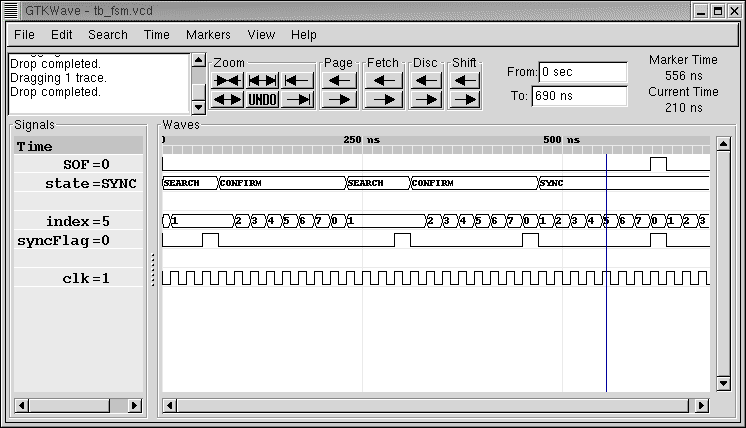
\includegraphics{tbfsm.png}
\fi

Signals are dumped in a suitable format. This format is inferred at
the \class{Signal} construction time, from the type of the initial
value. In particular, \class{bool} signals are dumped as single
bits. (This only works starting with Python2.3, when \class{bool} has
become a separate type).  Likewise, \class{intbv} signals with a
defined bit width are dumped as bit vectors. To support the general
case, other types of signals are dumped as a string representation, as
returned by the standard \function{str()} function.

\begin{notice}[warning]
Support for literal string representations is not part of the VCD
standard. It is specific to \program{gtkwave}. To generate a
standard VCD file, you need to use signals with a defined bit width
only.
\end{notice}


\section{High level modeling \label{model-hl}}

\begin{quote}
\em 
High level modeling is the ideal application of \myhdl{} and Python.
The possibilities are extensive and beyond the scope of most other
languages. It can be expected that \myhdl\ users will often have the
``Pythonic experience'' of finding an elegant solution to a complex
modeling problem.  The following section should be seen as a starting
point for experiments and exploration. Over time, more techniques that
prove useful will be added.
\end{quote}

\subsection{Modeling memories with built-in types \label{model-mem}}

Python has powerful built-in data types that can be useful to model
hardware memories. This can be merely a matter of putting an interface
around some data type operations.

For example, a \dfn{dictionary} comes in handy to model sparse memory
structures. (In other languages, this data type is called 
\dfn{associative array}, or \dfn{hash table}.) A sparse memory is one in
which only a small part of the addresses is used in a particular
application or simulation. Instead of statically allocating the full
address space, which can be large, it is better to dynamically
allocate the needed storage space. This is exactly what a dictionary
provides. The following is an example of a sparse memory model:

\begin{verbatim}


def sparseMemory(dout, din, addr, we, en, clk):
    """ Sparse memory model based on a dictionary.

    Ports:
    dout -- data out
    din -- data in
    addr -- address bus
    we -- write enable: write if 1, read otherwise
    en -- interface enable: enabled if 1
    clk -- clock input
    
    """
    memory = {}
    while 1:
        yield posedge(clk)
        if not en:
            continue
        if we:
            memory[addr] = din.val
        else:
            dout.next = memory[addr]
\end{verbatim} 

Note how we use the \code{val} attribute of the \code{din} signal, as
we don't want to store the signal object itself, but its current
value. (In many cases, \myhdl\ can use a signal's value automatically
when there is no ambiguity: for example, this happens whenever a
signal is used in expressions. When in doubt, you can always use the
\code{val} attribute explicitly.)

As a second example, we will demonstrate how to use a list to model a
synchronous fifo:

\begin{verbatim}
def fifo(dout, din, re, we, empty, full, clk, maxFilling=sys.maxint):
    """ Synchronous fifo model based on a list.

    Ports:
    dout -- data out
    din -- data in
    re -- read enable
    we -- write enable
    empty -- empty indication flag
    full -- full indication flag
    clk -- clock input
    Optional parameter:
    maxFilling -- maximum fifo filling, "infinite" by default

    """
    memory = []
    while 1:
        yield posedge(clk)
        if we:
            memory.insert(0, din.val)
        if re:
            dout.next = memory.pop()
        filling = len(memory)
        empty.next = (filling == 0)
        full.next = (filling == maxFilling)
\end{verbatim}

Again, the model is merely a \myhdl\ interface around some operations
on a list: \function{insert()} to insert entries, \function{pop()} to
retrieve them, and \function{len()} to get the size of a Python
object.

\subsection{Modeling errors using exceptions \label{model-err}}

In the previous section, we used Python data types for modeling. If
such a type is used inappropriately, Python's run time error system
will come into play. For example, if we access an address in the
\function{sparseMemory} model that was not initialized before, we will
get a traceback similar to the following (some lines omitted for
clarity):

\begin{verbatim}
Traceback (most recent call last):
...
  File "sparseMemory.py", line 30, in sparseMemory
    dout.next = memory[addr]
KeyError: 51
\end{verbatim}

Similarly, if the \code{fifo} is empty, and we attempt to read from
it, we get:

\begin{verbatim}
Traceback (most recent call last):
...
  File "fifo.py", line 34, in fifo
    dout.next = memory.pop()
IndexError: pop from empty list
\end{verbatim}

Instead of these low level errors, it may be preferable to define
errors at the functional level. In Python, this is typically done by
defining a custom \code{Error} exception, by subclassing the standard
\code{Exception} class. This exception is then raised explicitly when
an error condition occurs.

For example, we can change the \function{sparseMemory} function as
follows (with the doc string is omitted for brevity):

\begin{verbatim}
class Error(Exception):
    pass

def sparseMemory(dout, din, addr, we, en, clk):
    memory = {}
    while 1:
        yield posedge(clk)
        if not en:
            continue
        if we:
            memory[addr] = din.val
        else:
            try:
                dout.next = memory[addr]
            except KeyError:
                raise Error, "Uninitialized address %s" % hex(addr)
\end{verbatim}

This works by catching the low level data type exception, and raising
the custom exception with an appropriate error message instead.  If
the \function{sparseMemory} function is defined in a module with the
same name, an access error is now reported as follows:

\begin{verbatim}
Traceback (most recent call last):
...
  File "sparseMemory.py", line 57, in sparseMemory
    raise Error, "Uninitialized address %s" % hex(addr)
__main__.Error: Uninitialized address 0x33
\end{verbatim}

Likewise, the \function{fifo} function can be adapted as follows, to
report underflow and overflow errors:

\begin{verbatim}
class Error(Exception):
    pass

def fifo(dout, din, re, we, empty, full, clk, maxFilling=sys.maxint):
    memory = []
    while 1:
        yield posedge(clk)
        if we:
            memory.insert(0, din.val)
        if re:
            try:
                dout.next = memory.pop()
            except IndexError:
                raise Error, "Underflow -- Read from empty fifo"
        filling = len(memory)
        empty.next = (filling == 0)
        full.next = (filling == maxFilling)
        if filling > maxFilling:
            raise Error, "Overflow -- Max filling %s exceeded" % maxFilling
\end{verbatim}

In this case, the underflow error is detected as before, by catching a
low level exception on the list data type. On the other hand, the
overflow error is detected by a regular check on the length of the
list.


\subsection{Object-oriented modeling \label{model-obj}}

The models in the previous sections used high-level built-in data
types internally. However, they had a conventional RTL-style
interface.  Communication with such a module is done through signals
that are attached to it during instantiation.

A more advanced approach is to model hardware blocks as
objects. Communication with objects is done through method calls.
A method encapsulates all details of a certain task performed
by the object. As an object has a method interface instead
of an RTL-style hardware interface, this is a much 
higher level approach.

As an example, we will design a synchronized queue object. 
Such an object can be filled by producer, and independently
read by a consumer. When the queue is empty, the consumer
should wait until an item is available. The queue can be modeled
as an object with a \method{put(item)} and a \method{get()}
method, as follows:

\begin{verbatim}
from myhdl import *

def trigger(event):
    event.next = not event

class queue:
    def __init__(self):
       self.l = []
       self.sync = Signal(0)
       self.item = None
    def put(self,item):
       # non time-consuming method
       self.l.append(item)
       trigger(self.sync)
    def get(self):
       # time-consuming method
       if not self.l:
          yield self.sync
       self.item = self.l.pop(0)
\end{verbatim}

The \class{queue} object constructor initializes an internal list to
hold items, and a \var{sync} signal to synchronize the operation
between the methods. Whenever \method{put()} puts an item in the
queue, the signal is triggered.  When the \method{get()} method sees
that the list is empty, it waits on the trigger first.
\method{get()} is a generator method because 
it may consume time. As the \code{yield} statement is used in \myhdl\
for timing control, the method cannot ``yield'' the item. Instead, it
makes it available in the \var{item} instance variable.

To test the queue operation, we will model a producer and a consumer
in the test bench.  As a waiting consumer should not block a whole
system, it should run in a concurrent ``thread''. As always in
\myhdl{}, concurrency is modeled by Python generators. Producer
and consumer will thus run independently, and we will monitor
their operation through some print statements:

\begin{verbatim}
q = queue()

def Producer(q):
    yield delay(120)
    for i in range(5):
        print "%s: PUT item %s" % (now(), i)
        q.put(i)
        yield delay(max(5, 45 - 10*i))

def Consumer(q):
    yield delay(100)
    while 1:
        print "%s: TRY to get item" % now()
        yield q.get()
        print "%s: GOT item %s" % (now(), q.item)
        yield delay(30)

def main():
    P = Producer(q)
    C = Consumer(q)
    return P, C 

sim = Simulation(main())
sim.run()
\end{verbatim}

Note that the generator method \method{get()} is called in a
\code{yield} statement in the \function{Consumer} function. The new
generator will take over from \function{Consumer}, until it is done.
Running this test bench produces the following output:

\begin{verbatim}
% python queue.py
100: TRY to get item
120: PUT item 0
120: GOT item 0
150: TRY to get item
165: PUT item 1
165: GOT item 1
195: TRY to get item
200: PUT item 2
200: GOT item 2
225: PUT item 3
230: TRY to get item
230: GOT item 3
240: PUT item 4
260: TRY to get item
260: GOT item 4
290: TRY to get item
StopSimulation: No more events
\end{verbatim}
